% !TeX spellcheck = en_US
\documentclass[12pt]{report}
\usepackage[a4paper, total={7in, 9in}]{geometry}
\usepackage{setspace} %Line spacing
\onehalfspacing

\usepackage{pdfpages}

\usepackage{fancyhdr}
\usepackage{lastpage}

% For the chapters not to modify the page style
\usepackage{titlesec}
\titleformat{\chapter}{\bfseries}{\huge\arabic{chapter}.}{10pt}{\huge}
\titleclass{\chapter}{straight}

%REFERENCES
\usepackage{siunitx, multirow, booktabs}
\usepackage{blindtext,alltt}
\usepackage[backend=bibtex, style=numeric, sorting=none, locallabelwidth]{biblatex}
\addbibresource{/home/leonidas/Documents/References.bib}

\usepackage{listings}

\usepackage{wrapfig}
\usepackage{array}
\usepackage{multicol}
\usepackage{url}
\usepackage[nottoc]{tocbibind} %Add references to index.
\usepackage{amsmath, amssymb}
\usepackage{upgreek, dsfont, mathrsfs}
\usepackage{stmaryrd}


\usepackage[breakable]{tcolorbox}
\usepackage{parskip} % Stop auto-indenting (to mimic markdown behaviour)


% Basic figure setup, for now with no caption control since it's done
% automatically by Pandoc (which extracts ![](path) syntax from Markdown).
\usepackage{graphicx}
\usepackage{caption}

%Footnoe symbol instead of numbers
%1   asterisk        *   2   dagger      †   3   double dagger       ‡
%4   section symbol  §   5   paragraph   ¶   6   parallel lines      ‖
%7   two asterisks   **  8   two daggers ††  9   two double daggers  ‡‡
\usepackage[symbol]{footmisc}
\renewcommand{\thefootnote}{\fnsymbol{footnote}}

\usepackage{float}
\floatplacement{figure}{H} % forces figures to be placed at the correct location

\usepackage{xcolor} % Allow colors to be defined
\usepackage{enumerate} % Needed for markdown enumerations to work
\usepackage{geometry} % Used to adjust the document margins
\usepackage{amsmath} % Equations
\usepackage{amssymb} % Equations
\usepackage{textcomp} % defines textquotesingle
% Hack from http://tex.stackexchange.com/a/47451/13684:
\AtBeginDocument{%
	\def\PYZsq{\textquotesingle}% Upright quotes in Pygmentized code
}
\usepackage{upquote} % Upright quotes for verbatim code
\usepackage{eurosym} % defines \euro

\usepackage{iftex}
\ifPDFTeX
\IfFileExists{alphabeta.sty}{
	\usepackage{alphabeta}
}{
	\usepackage[mathletters]{ucs}
	\usepackage[utf8x]{inputenc}
}
\else
\usepackage{fontspec}
\usepackage{unicode-math}
\fi


% The hyperref package gives us a pdf with properly built
% internal navigation ('pdf bookmarks' for the table of contents,
% internal cross-reference links, web links for URLs, etc.)
\usepackage{hyperref}
% The default LaTeX title has an obnoxious amount of whitespace. By default,
% titling removes some of it. It also provides customization options.
\usepackage{titling}
\usepackage{longtable} % longtable support required by pandoc >1.10
\usepackage{booktabs}  % table support for pandoc > 1.12.2
\usepackage{array}     % table support for pandoc >= 2.11.3
\usepackage{calc}      % table minipage width calculation for pandoc >= 2.11.1
\usepackage[inline]{enumitem} % IRkernel/repr support (it uses the enumerate* environment)
\usepackage[normalem]{ulem} % ulem is needed to support strikethroughs (\sout)
% normalem makes italics be italics, not underlines
\usepackage{mathrsfs}



% Colors for the hyperref package
\definecolor{urlcolor}{rgb}{0,.145,.698}
\definecolor{linkcolor}{rgb}{.71,0.21,0.01}
\definecolor{citecolor}{rgb}{.12,.54,.11}

% ANSI colors
\definecolor{ansi-black}{HTML}{3E424D}
\definecolor{ansi-black-intense}{HTML}{282C36}
\definecolor{ansi-red}{HTML}{E75C58}
\definecolor{ansi-red-intense}{HTML}{B22B31}
\definecolor{ansi-green}{HTML}{00A250}
\definecolor{ansi-green-intense}{HTML}{007427}
\definecolor{ansi-yellow}{HTML}{DDB62B}
\definecolor{ansi-yellow-intense}{HTML}{B27D12}
\definecolor{ansi-blue}{HTML}{208FFB}
\definecolor{ansi-blue-intense}{HTML}{0065CA}
\definecolor{ansi-magenta}{HTML}{D160C4}
\definecolor{ansi-magenta-intense}{HTML}{A03196}
\definecolor{ansi-cyan}{HTML}{60C6C8}
\definecolor{ansi-cyan-intense}{HTML}{258F8F}
\definecolor{ansi-white}{HTML}{C5C1B4}
\definecolor{ansi-white-intense}{HTML}{A1A6B2}
\definecolor{ansi-default-inverse-fg}{HTML}{FFFFFF}
\definecolor{ansi-default-inverse-bg}{HTML}{000000}

% common color for the border for error outputs.
\definecolor{outerrorbackground}{HTML}{FFDFDF}

% Prevent overflowing lines due to hard-to-break entities
\sloppy 
% Setup hyperref package
\hypersetup{
	breaklinks=true,  % so long urls are correctly broken across lines
	colorlinks=true,
	urlcolor=urlcolor,
	linkcolor=linkcolor,
	citecolor=citecolor,
}

\definecolor{codegreen}{rgb}{0,0.6,0}
\definecolor{codegray}{rgb}{0.5,0.5,0.5}
\definecolor{codepurple}{rgb}{0.58,0,0.82}
\definecolor{backcolour}{rgb}{0.95,0.95,0.92}

\lstdefinestyle{mystyle}{
	backgroundcolor=\color{backcolour},   
	commentstyle=\color{codegreen},
	keywordstyle=\color{magenta},
	numberstyle=\tiny\color{codegray},
	stringstyle=\color{codepurple},
	basicstyle=\ttfamily\footnotesize,
	breakatwhitespace=false,         
	breaklines=true,                 
	captionpos=b,                    
	keepspaces=true,                 
	numbers=left,                    
	numbersep=5pt,                  
	showspaces=false,                
	showstringspaces=false,
	showtabs=false,                  
	tabsize=2
}

\lstset{style=mystyle}

\pagestyle{fancy}
\fancyhf{}
\rhead{}
\lhead{THESIS PROJECT $|$ \textcolor{red}{MONITORED HIVES FOR HONEYBEES}}
\lfoot{Universidad Autónoma de Chihuahua}
\rfoot{Page \thepage \hspace{1pt} of \pageref{LastPage}}

\renewcommand{\headrulewidth}{0.5pt} %ancho de la recta del encabezado superior


\begin{document}
	
	%\thispagestyle{empty}
	\begin{titlepage}
		\begin{center}
			\begin{tabular}{c}
				
\includegraphics[scale=0.2]{BN_uach.png}\\[3.5ex]
				\textbf{\LARGE Universidad Autónoma de Chihuahua}\\[3.5ex]
				\textbf{\Large Facultad de Ingeniería}\\[3.5ex]
				\hline\\[3ex]
				\begin{minipage}{17cm}
					\centering
					\begin{doublespace}
						\textbf{\LARGE MONITORED HIVES FOR HONEYBEES: Implementing a Microphone on the Monitoring Device}
					\end{doublespace}
				\end{minipage}\\[3.5ex]
				\hline
			\end{tabular}\vfill
			{\large Thesis Protocol.}\\\vfill
			{\large \textbf{Student:} Leonardo Rafael León Mora.}\\\vfill
			{\large \textbf{Thesis director:} Dr. Daniel Espinobarro Velázquez.}\\\vfill
			{\large \textbf{Suggested advisors:}}\\[3.5ex]
			\begin{itemize}
				\item {\large M.C. Carlos Hugo Larrinúa Pacheco.}\\[3.5ex]
				\item {\large M.I. Joseph Isaac Ramírez Hernández.}\\[3.5ex]
			\end{itemize}
			\vfill
			{\large \textbf{Chihuahua, Chih.,} \today.}\\[3.5ex]
		\end{center}
	\end{titlepage}
	
	
	%------------------------------------------------------------------------------------------
	% 1. ANTECEDENTES.
	%------------------------------------------------------------------------------------------
	
	\chapter{BACKGROUND}
	
	Cada vez que se revisa la colmena de forma manual existe la posiblidad de matar a la reina al extraer uno de los bastidores de la colmena, lo que puede llevar a la perdida total de la misma.
	
	\section{Dániel Tamás Várkonyi - Dynamic noise filtering for multi-class classification of beehive audio data}
	
	In the majority of apiaries, identification of the health condition of a bee colony is done manually by opening and inspecting the hive. Opening the hive, however, introduces certain stress to the colony while changing the micro-climate within the hive. Afterward, bees have to expend considerable energy to re-establish the equilibrium within the beehive. Consequently, \textbf{frequent manual inspection of a hive reduces the amount of honey the given bee colony produces}.
	
	\par Analyzing the colony's sound might reveal certain anomalous events within the hive, like the presence of an intruder or \textbf{the preparation of the colony for swarming}. The first technological approaches used for monitoring bees' condition via audio analysis were conducted in the late 20th century using spectral analysis in the range of $0-3$ kHz \cite{dietlein1985spectral_analysis}.
	
	\par Applying machine learning ({\tt ML}) to audio analysis for bee queen presence detection and swarming prediction leads to a basic binary classification task, i. e. predicting if the queen is present or not and if the colony is swarming or not. Moreover, \textbf{the sound of a bee colony in a ``queenless'' or swarming state is well distinguishable from its sounds when a queen is present or the colony is not swarming} \cite{allen1956behaviourbeeswarming, hord2013behavioraudioanalysis}. \textbf{The stress level of the colony exposed to an ``anomaly'' likely implies a substantially different sound from the one when being in a normal state}.\\
	An important issue, contravening the approaches found in the literature, is that \textbf{these problems might not necessarily correspond to binary classification tasks}. For example, identification of various (more than two) types of diseases, intrusion detection by different pests, or estimation of exposure of bees to diverse palettes of chemicals, naturally, calls for multi-label or even multi-class approaches. An assumption here, posing possible difficulties for application of ML techniques, is that \textbf{bee sounds corresponding to various classes (labels) might not be so easily distinguishable from each other} as they usually are in the before mentioned binary cases where ``anomalous'' and ``normal'' states are well-detectable even for humans.
	
	\begin{figure}
		\centering
		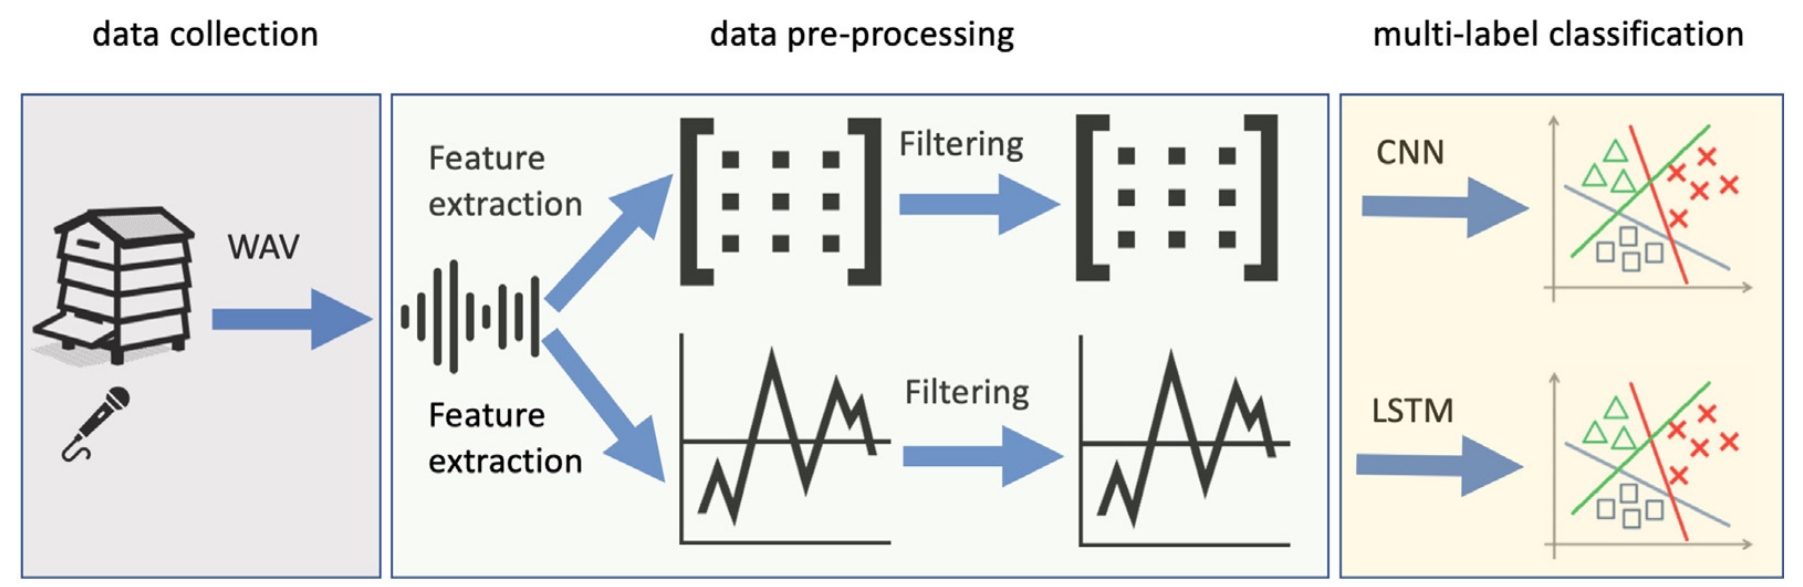
\includegraphics[scale = 0.25]{beeaudioworkflow.png}
		\caption{A general audio data analytics workflow used in our experiments.}
		\label{fig:audioworkflow}
	\end{figure}
	
	\par There is a huge gap int he literature considering multi-label or multi-class classification of bee audio data. According to our knowledge. The only work related to multi-label bee sound classification \cite{gradivsek2017predictingbumblebees}, is focused on identifying 12 bumblebee species from their buzzing sounds (from a small-scale dataset using traditional {\tt ML} techniques, such that naïve Bayes decision trees, support vector machines, and random forests).
	
	\begin{itemize}
		\item \textbf{Problem \# 1}. The classification accuracy of the audio data analytics work flow, shown in figure \ref{fig:audioworkflow}, does not only depend on the discriminative power of the used {\tt ML} techniques, but also, on the used pre-processing steps. One of the basics problems of audio signals is that, even after filtering out irrelevant information, the resulting data represented as time-series have very high dimensionality. Feature extraction ({\tt FE}) methods are utilized to extract and represent the most important features within the audio signal in a compact form (time-series or spectrograms), preserving a significant portion of its original information content. After {\tt FE}, {\tt ML} techniques can be applied on the data (depending on the amount, dimensionality and the task intended to be solved).
		
		\item \textbf{Problem \# 2}. According to our knowledge, there is no reference in the literature to a survey comparing various combinations of audio {\tt FE} (image or time-series), noise filtering ({\tt NF}) and {\tt ML} (image or time-series classification) techniques for bee sound analytics. including thorough hyper-parameter ({\tt HP}) tuning and validation procedures as well as utilizing large datasets.
		
		\item \textbf{Problem \# 3}. According to our knowledge, there is no large-scale publicly available bee sound benchmark data suitable for research on multi-label or multi-class bee sound classification approaches.\\
		Several {\tt ML} developments, e.g. various deep learning ({\tt DL}) models, have been developed working efficiently on specific problems related to audio processing like, for example, human speech recognition. However, our experiments showed that \textbf{these methods are not performing well in case of a multi-label bee sound classification problem} in which the difference between various classes is inconspicuous.
		
		\item \textbf{Problem \# 4}. The main reason for the poor performance of state-of-the-art {\tt ML} models for multi-label bee sound classification lies in the poor performance of the used {\tt NF} methods, which seems to be not suitable for bee sound data.
	\end{itemize}
	
	
	
	
	%------------------------------------------------------------------------------------------
	% 2. JUSTIFICACIÓN.
	%------------------------------------------------------------------------------------------
	
	\chapter{JUSTIFICACIÓN}
	
	
	%------------------------------------------------------------------------------------------
	% 3. LA PROPUESTA Y LA CARRERA.
	%------------------------------------------------------------------------------------------
	
	\chapter{RELACIÓN DE LA PROPUESTA CON LAS MATERIAS DE LA CARRERA}
	
	
	%------------------------------------------------------------------------------------------
	% 4. OBJETIVOS.
	%------------------------------------------------------------------------------------------
	
	\chapter{OBJETIVOS}
	
	
	%------------------------------------------------------------------------------------------
	% 5. HIPÓTESIS.
	%------------------------------------------------------------------------------------------
	
	\chapter{HIPÓTESIS}
	
	
	
	%------------------------------------------------------------------------------------------
	% 6. METODOLOGÍA.
	%------------------------------------------------------------------------------------------
	
	\chapter{METODOLOGÍA}
	
	
	%------------------------------------------------------------------------------------------
	% 7. PLAN DE TRABAJO.
	%------------------------------------------------------------------------------------------
	
	\chapter{PLAN DE TRABAJO}
	
	
	
	%------------------------------------------------------------------------------------------
	% 8. LUGAR DE DESARROLLO.
	%------------------------------------------------------------------------------------------
	
	\chapter{LUGAR DE DESARROLLO}
	
	
	
	%------------------------------------------------------------------------------------------
	% 9. BIBLIOGRAFÍA.
	%------------------------------------------------------------------------------------------
	\pagebreak
	\addcontentsline{toc}{chapter}{BIBLIOGRAPHY}
	\printbibliography
	\thispagestyle{empty}
	
\end{document}